\documentclass[a4paper,11pt]{book}
\usepackage{import}
\usepackage{preamb}

\makeindex

\begin{document}

\small
\begin{multicols}{3}

%\maketitle

\thispagestyle{empty}
\scriptsize
\newpage


\begin{subbox}{subbox}{}
\centering
\Large{\textbf{Network Science   \\ Cheatsheet}}
\end{subbox}

\begin{multibox}{2}
\begin{subbox}{subbox}{}
\centering

\includegraphics[width=0.8\textwidth]{pics/logo.png}
\end{subbox}
\begin{subbox}{subbox}{}
\centering
Made by \\
\large{
Remy Cazabet
}
\end{subbox}
\end{multibox}
% \section{Blocks and Community structure}


\begin{subbox}{subbox}{}
\centering
\Large{\textbf{Network Science -  Introduction}}
\end{subbox}


\begin{textbox}{Networks: Graph notation}
Graph notation : $G=(V,E)$

\begin{tabular}{p{0.2\textwidth}|p{0.8\textwidth}}\scriptsize


 $V$ & set of vertices/nodes. \\
 $E$ &  set of edges/links. \\
 $u\in V$ & a node. \\
 $(u,v) \in E$ & an edge. \\
\end{tabular}
\end{textbox}






























\begin{textbox}{Network - Graph notation}
\begin{multibox}{2}
\begin{subbox}{white}{\textcolor{black}{Graph}}
\centering
%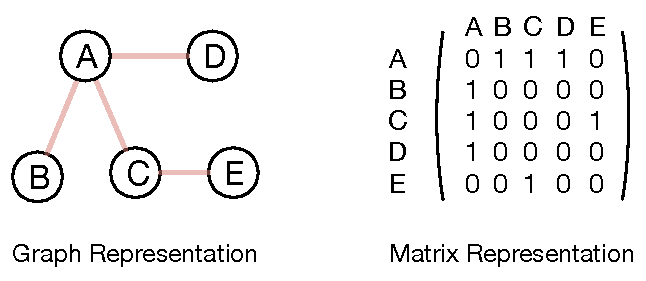
\includegraphics[width=\textwidth]{CheatSheet_pic.pdf}
\adjustbox{width=0.9\textwidth }{
%\scalebox{1}[0.5]{
%\rotatebox[90]{
\begin{tikzpicture}[scale=0.3,rotate=0][every node/.style={inner sep=0,outer sep=0}]
\clip (0,-0.5) rectangle (6,6.5);
\Vertex[x=1.781,y=1.331,size=0.3,opacity=0.8,label=1]{0}
\Vertex[x=3.083,y=3.151,size=0.3,opacity=0.8,label=2]{1}
\Vertex[x=2.831,y=0.200,size=0.3,opacity=0.8,label=6]{5}
\Vertex[x=4.058,y=1.136,size=0.3,opacity=0.8,label=5]{4}
\Vertex[x=4.219,y=5.643,size=0.3,opacity=0.8,label=3]{2}
\Vertex[x=2.386,y=5.800,size=0.3,opacity=0.8,label=4]{3}
\Edge[](0)(1)
\Edge[](0)(5)
\Edge[](0)(4)
\Edge[](1)(2)
\Edge[](1)(3)
\Edge[](1)(4)
\Edge[](1)(5)
\Edge[](5)(4)
\Edge[](4)(4)
\Edge[](2)(3)
\end{tikzpicture}
}%\end{resizebox}
\end{subbox}
\begin{subbox}{white}{\textcolor{black}{Graph notation}}
\[
G=(V,E)
\]
\[
V=\{1,2,3,4,5,6\}
\]
\[
\begin{split}
E=\{(1, 2),
 (1, 6),\\
 (1, 5),
 (2, 4),
 (2, 3),
 (2, 5),\\
 (2, 6),
 (6, 5),
 (5, 5),
 (4, 3)\}
 \end{split}
\]
\end{subbox}

\end{multibox}
\end{textbox}












\begin{textbox}{Types of networks}

\textbf{Simple graph}: Edges can only exist or not exist between each pair of node, and there are no self-loops, i.e., an edge connecting a node to itself.

\textbf{Directed graph}: Edges have a direction: $(u,v)\in V$ does not imply $(v,u)\in V$ 

\textbf{Weighted graph}: A weight is associated to every edge. 

    
\noindent\rule{4cm}{0.1pt}

\tiny{
Other types of graphs (multigraphs, multipartite, hypergraphs, etc.) are introduced later}


\end{textbox}












\begin{textbox}{Counting nodes and edges}

\begin{tabular}{p{0.07\textwidth}|p{0.8\textwidth}}\scriptsize
$N,n$ & \textbf{size}: number of nodes $|V|$.  \\

$L,m$ & number of edges $|E|$\\
$L_{max}$ & Maximum number of links
\[  \text{Undirected network: } {N\choose 2 }=N(N-1)/2
\]
\[
 \text{Directed network: }=N(N-1)
\]

\end{tabular}

\end{textbox}










\begin{textbox}{Node-Edge description}
\begin{tabular}{p{0.1\textwidth}|p{0.8\textwidth}}\scriptsize

$N_u$ & \textbf{Neighbourhood} of $u$, nodes sharing a link with $u$. \\


$k_u$ & \textbf{Degree} of $u$, number of neighbors $|N_u|$. \\
\hline
$N^{out}_u$ & \textbf{Successors} of $u$, nodes such as $(u,v)\in E$ in a directed graph \\

$N^{in}_u$ & \textbf{Predecessors} of $u$, nodes such as $(v,u)\in E$ in a directed graph \\

$k^{out}_u$ & \textbf{Out-degree} of $u$, number of outgoing edges  $|N^{out}_u|$. \\

$k^{in}_u$ & \textbf{In-degree} of $u$, number of incoming edges $|N^{in}_u|$ \\

\hline

$w_{u,v}$ & \textbf{Weight} of edge $(u,v)$. \\

$s_u$ & \textbf{Strength} of $u$, sum of weights of adjacent edges, $s_u = \sum_v w_{uv}$. \\
\end{tabular}

\end{textbox}














\begin{textbox}{Network descriptors - Nodes/Edges}
\begin{tabular}{p{0.08\textwidth}|p{0.8\textwidth}}\scriptsize

$\langle k \rangle$ & \textbf{Average degree}:
Real networks are sparse, i.e., typically $\langle k \rangle \ll n$. Increases slowly with network size, e.g., $\langle k \rangle \sim \log(n)$ \footcite{leskovec2005graphs}

\[\langle k \rangle=\frac{2m}{n}\]\\

$d,d(G)$ & \textbf{Density}: Fraction of pairs of nodes connected by an edge in $G$.

\[d=L/L_{\max}
\]\\

\end{tabular}
\end{textbox}
















\begin{textbox}{Paths - Walks - Distance}
\textbf{Walk}: Sequences of adjacent edges or nodes (e.g., \textbf{1.2.1.6.5} is a valid walk)

\textbf{Path}: a walk in which each node is distinct.

\textbf{Path length}: number of \textbf{edges} encountered in a path

\textbf{Weighted Path length}: Sum of the weights of edges on a path


\textbf{Shortest path}: The shortest path between nodes $u,v$ is a path of minimal \textit{path length}. Not necessarily unique.

\textbf{Weighted Shortest path}: path of minimal \textit{weighted path length}.


\textbf{$\ell_{u,v}$: Distance}: The distance between nodes $u,v$ is the length of the shortest path


\end{textbox}






















\begin{textbox}{Network descriptors - Paths}
\begin{tabular}{p{0.07\textwidth}|p{0.8\textwidth}}\scriptsize





$\ell_{\max}$ & \textbf{Diameter}: maximum \textit{distance} between any pair of nodes.\\


$\langle \ell \rangle$ & \textbf{Average distance}:
\[
\langle \ell \rangle = \frac{1}{n(n-1)}\sum_{i\neq j} \ell_{ij}
\]\\

\end{tabular}

\end{textbox}










\begin{textbox}{Degree distribution}

The degree distribution is considered an important network property. They can follow two typical distributions: 
\begin{itemize}
    \item \textbf{Bell-curved} shaped (Normal/Poisson/Binomial)
    \item \textbf{Scale-free}, also called \textit{Power-law}
\end{itemize}
A Bell-curved distribution has a \textit{typical scale}: as human height, it is centered on an average value. A Scale-free distribution has no typical scale: as human wealth, its average value is not representative, low values (degrees) are the most frequent, while a few very large values can be found (hubs, large degree nodes). It has a \textit{long tail}, meaning that rare (large) values are not as rare as in a bell-curved distribution. 

\centering
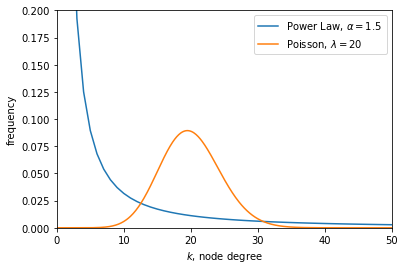
\includegraphics[width=0.7\textwidth]{pics/distribution.png}


\noindent\rule{4cm}{0.1pt}

\tiny{
More details later.}
\end{textbox}






\begin{textbox}{Subgraphs}

\textbf{Subgraph $H(W)$} (induced subgraph): subset of nodes $W$ of a graph $G=(V,E)$ and edges connecting them in $G$, i.e., subgraph $H(W)=(W,E'), W \subset V, (u,v) \in E' \iff u,v \in W \wedge (u,v) \in E$

\textbf{Clique}: subgraph with $d=1$

\textbf{Triangle}: clique of size 3

\textbf{Connected component}: a subgraph in which any two vertices are connected to each other by paths, and which is connected to no additional vertex in the supergraph

\textbf{Strongly Connected component}: In directed networks, a subgraph in which any two vertices are connected to each other by paths

\textbf{Weakly Connected component}: In directed networks, a subgraph in which any two vertices are connected to each other by paths if we disregard directions

\end{textbox}


\begin{textbox}{Triangles counting}

$\delta_u$ - \textbf{Triads of $u$:} number of triangles containing node $u$

$\Delta$ - \textbf{Number of triangles in the graph} total number of triangles in the graph, $\Delta=\frac{1}{3}\sum_{u\in V}\delta_u$. 

\begin{subbox}{subbox}{}
\tiny{Each \textbf{triangle} in the graph is counted as a \textbf{triad} once by each of its nodes. }
\end{subbox}

$\delta^{\max}_u$ - \textbf{Triad potential of $u$:} maximum number of triangles that could exist around node $u$, given its degree: $\delta^{\max}_u=\binom {k_{u}}{2}$

$\Delta^{\max}$ - \textbf{Triangle potential of G:} maximum number of triangles that could exist in the graph, given its degree distribution: $\Delta^{\max}=\frac {1}{3}\sum_{u\in V}\ \delta^{\max} (u)$


\end{textbox}












\begin{textbox}{Clustering Coefficents - Triadic closure}
The clustering coefficient is a measure of the triadic closure of a network or of a node neighborhood. The triadic closure is a notion coming from social network analysis, often summarized by the aphorism \textit{The friends of my friends are my friends}. 

\noindent\rule{4cm}{0.1pt}


$C_u$ - \textbf{Node clustering coefficient:} density of the subgraph induced by the neighborhood of $u$, $C_u = d(H(N_u)$. Also interpreted as the fraction of all possible triangles in $N_u$ that exist, $\frac{\delta_u}{\delta^{\max}_u}$

$\langle C \rangle$ - \textbf{Average clustering coefficient:} Average clustering coefficient of all nodes in the graph, $\bar C = \frac{1}{N}\sum_{u \in V} C_u$.\\ 

\begin{subbox}{subbox}{}
\tiny{Be careful when interpreting this value, since all nodes contributes equally, irrespectively of their degree, and that low degree nodes tend to be much more frequent than hubs, and their $C$ value is very sensitive, i.e., for a node $u$ of degree 2, $C_u \in \{0,1\}$, while nodes of higher degrees tend to have more contrasted scores.}
\end{subbox}

$C^g$ - \textbf{Global clustering coefficient:} Fraction of all possible triangles in the graph that do exist, $C^g= \frac{\Delta}{\Delta^{\max}} $

\end{textbox}



















\begin{textbox}{Small World Network}
A network is said to have the \textbf{small world} property when it has some structural properties\footcite{watts1998collective}. The notion is usually not quantitatively defined, but two properties are required:
\begin{itemize}
    \item Average distance must be short, i.e., $\langle\ell\rangle \approx \log(N)$
    \item Clustering coefficient must be high, i.e., much larger than in a random network , e.g., $C^g \gg d$, with $d$ the network density
\end{itemize}

This property is considered characteristic of \textit{real} networks, as opposed to random networks. It is believed to be associated to particular properties (robustness to failures, efficient information flow, etc.), and to be the consequence of emergent mechanisms typical of \textit{complex systems}.

\noindent\rule{4cm}{0.1pt}

Be careful: in some contexts, \textit{small world network} can be used for a network that has a small Average distance, without considering its Clustering Coefficient.
\end{textbox}








\begin{textbox}{Cores and Shells}

Many real networks are known to have a \textbf{core-periphery} structure, i.e., there is a densely connected core at its center and a more peripheral zone in which nodes are loosely connected between them and to the core.

\noindent\rule{4cm}{0.1pt}

\textbf{k-core:} The  k-core (core of order $k$) of $G(V,E)$ is the largest subgraph $H(C)$ such as all nodes have at least a degree $k$, i.e.,  $\forall u \in C, {k}^H_u \geq k$, with $k^H_u$ the degree of node $u$ in subgraph $H$.

\textbf{coreness:} A vertex $u$ has coreness $k$ if it belongs to the $k$-core but not to the $k+1$-core.

\textbf{c-shell:} all vertices whose coreness is exactly $c$.

\centering
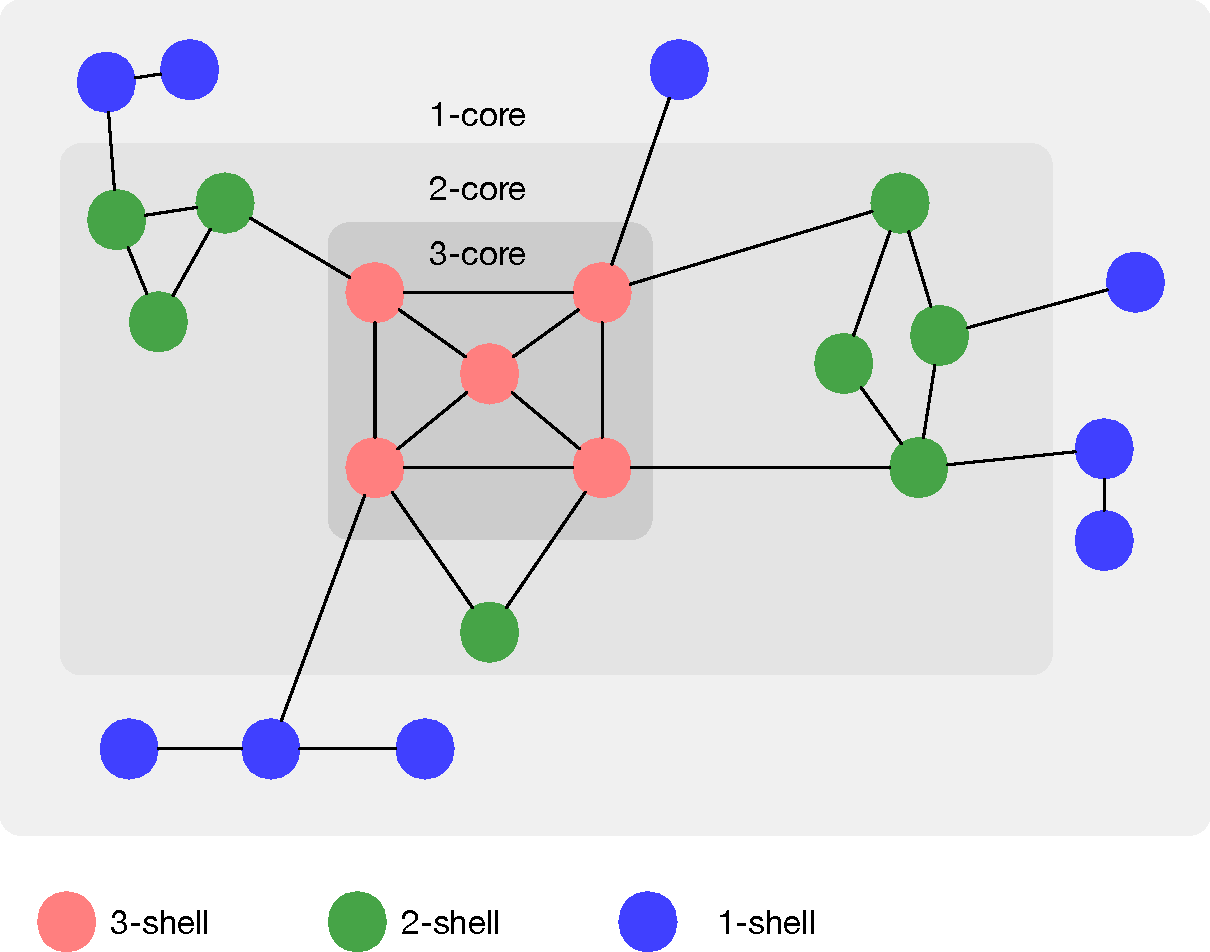
\includegraphics[width=0.7\textwidth]{pics/k-cores.pdf}

\end{textbox}














\begin{textbox}{Vocabulary}
\textbf{Singleton}: node with a degree $k=0$

\textbf{Hub}: node $u$ with $k_u \gg \langle k \rangle$

\noindent\rule{4cm}{0.1pt}

\textbf{Bridge}: Edge which, when removed, split a connected component in two.

\textbf{Self-loop}: Edge which connects a node to itself. 

\textbf{Stub}: A stub is an half edge, i.e., edge $(u,v)$ has a stub connected to $u$ and another connected to $v$.


\noindent\rule{4cm}{0.1pt}

\textbf{Complete network}: $L=L_{max}$

\textbf{Sparse network}: $d \ll 1$, $ L \ll L_{max}$

\textbf{Connected Graph}: Graph composed of a single connected component


\end{textbox}

\begin{textbox}{Going Further}

Books about network science as a whole:
\begin{itemize}
    \item\cite{barabasi2016network} (free)
    \item \cite{coscia2021atlas} (free)
    \item \cite{zinoviev2018complex}
    \item \cite{menczer2020first}
\end{itemize}

\end{textbox}

 \AtNextBibliography{\footnotesize}


\printbibliography[heading=subbibliography]


\end{multicols}



\end{document}

